% This is text associated with the open textbook "Open Electromagnetics"
% See immediately below for author, date
% This work is licensed under the Creative Commons Attribution-ShareAlike 4.0 International License. (CC BY SA 4.0) 
% To view a copy of the license, visit http://creativecommons.org/licenses/by-sa/4.0/

%ORB TITLE Magnetic Field Inside a Straight Coil
%ORB AUTHOR 0        # S.W. Ellingson, Virginia Tech (ellingson@vt.edu)
%ORB DATE 20180628   # yyyymmdd
%ORB ABSTRACT Magnetic Field Inside a Coil

\label{m0120_Magnetic_Field_of_a_Coil} % <-- Must match name of this file and module directory name.  Don't mess with this!
\index{coil|(}

In this section, we use the magnetostatic integral form of Ampere's Circuital Law 
\index{Ampere's law!magnetostatics}
(ACL) (Section~\ref{m0019_Amperes_Law_Magnetostatics}) to determine the magnetic field inside a straight coil of the type shown in Figure~\ref{m0120_fStraightCoil} in response to a steady (i.e., DC) current.
The result has a number of applications, including the analysis and design of inductors, 
\index{inductor}
solenoids 
\index{solenoid}
(coils that are used as magnets, typically as part of an actuator), and as a building block and source of insight for more complex problems.
%
\begin{figure}[b!]
\begin{center}
\pdftooltip{{  % note double braces
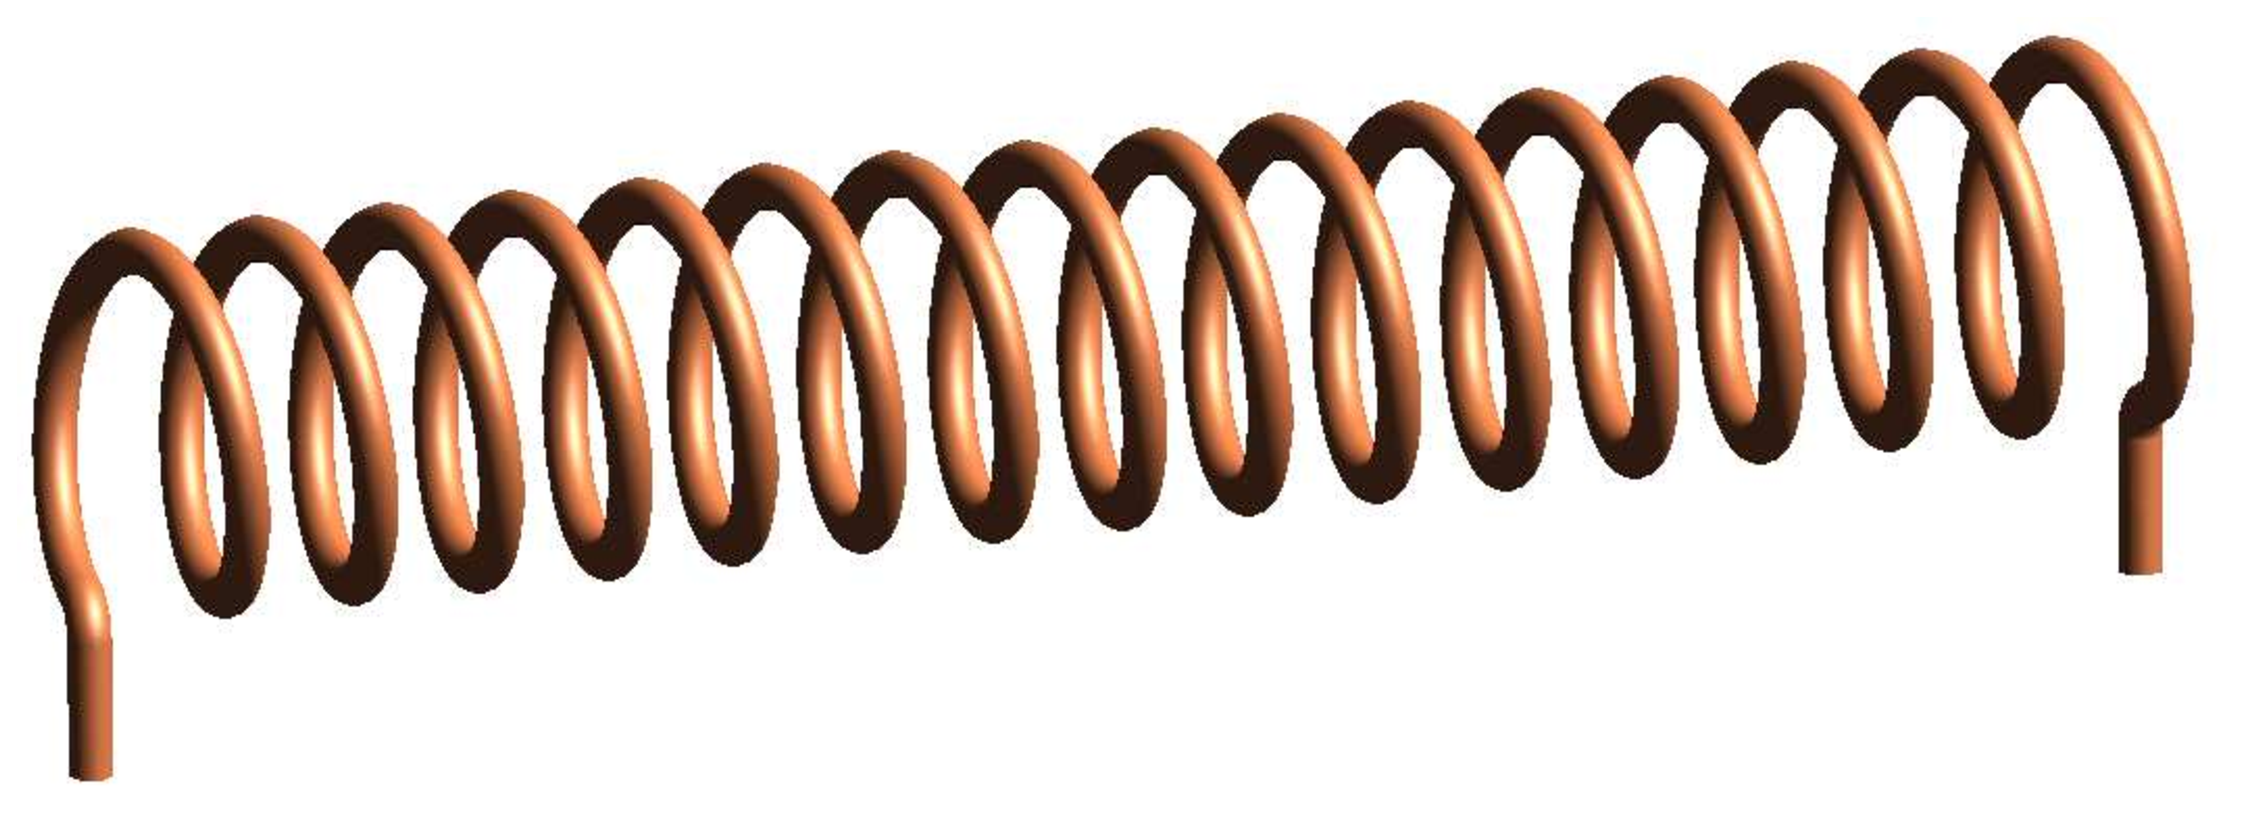
\includegraphics[width=1.5in]{modules/m0120_fStraightCoil.eps}
% https://en.wikipedia.org/wiki/File:Solenoid-1.png
}}{A circular coil, with uniform turns.}
\end{center} 
\centerline{\scriptsize 
by~\hyperref[m0120_fStraightCoil_Credit]{Zureks} (public domain)
%\href{https://creativecommons.org/licenses/by-sa/4.0/}{CC BY~SA 4.0} 
} 
\caption{
\label{m0120_fStraightCoil}
A straight coil.
}
\end{figure}  

The present problem is illustrated in Figure~\ref{m0120_fCoil}.
The coil is circular with radius $a$ and length $l$, and consists of $N$ turns (``windings'') of wire wound with uniform winding density.
Since the coil forms a cylinder, the problem is easiest to work in cylindrical coordinates with the axis of the coil aligned along the $z$ axis.
%
\begin{figure}
\begin{center}
\pdftooltip{{  % note double braces
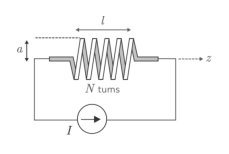
\includegraphics[width=2.5in]{modules/m0120_fCoil.eps}
}}{A circular coil with radius a and length l, consisting of N turns wound uniformly lies on the z-axis in a series circuit with current pointed to the right running counterclockwise.}
\end{center} 
% ***WikipediaCommonsURL
%\centerline{\scriptsize 
%\copyright~\hyperref[m0120_fCoil_Credit]{author} 
%\href{https://creativecommons.org/licenses/by-sa/4.0/}{CC BY-SA 4.0} 
%} 
\caption{
\label{m0120_fCoil}
Determination of the magnetic field due to DC current in a coil.
}
\end{figure}  

To begin, let's take stock of what we already know about the answer, which is actually quite a bit.
The magnetic field deep inside the coil is generally aligned with axis of the coil as shown in Figure~\ref{m0120_fStraightCoilFieldLines}.
This can be explained using the result for the magnetic field due to a straight line current (Section~\ref{m0119_Magnetic_Field_of_a_Long_Wire}), in which we found that the magnetic field follows a ``right-hand rule.'' 
\index{right-hand rule!magnetic field of a wire}
The magnetic field points in the direction of the fingers of the right hand when the thumb of the right hand is aligned in the direction of current flow. 
The wire comprising the coil is obviously \emph{not} straight, but we can consider just one short segment of one turn and then sum the results for all such segments.
When we consider this for a single turn of the coil, the situation is as shown in Figure~\ref{m0120_fOneTurn}.
Summing the results for many loops, we see that the direction of the magnetic field inside the coil must be generally in the $+\hat{\bf z}$ direction when the current $I$ is applied as shown in Figures~\ref{m0120_fCoil} and \ref{m0120_fStraightCoilFieldLines}.
However, there is one caveat. The windings must be sufficiently closely-spaced that the magnetic field lines can only pass through the openings at the end of the coil and  do not take any ``shortcuts'' between individual windings.
%
\begin{figure}
\begin{center}
\pdftooltip{{  % note double braces
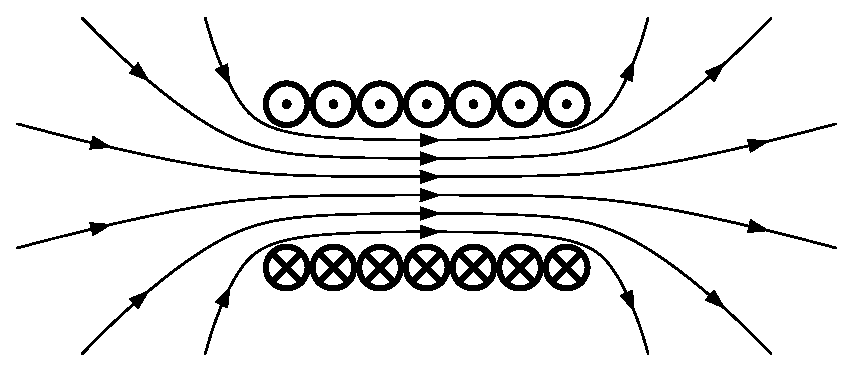
\includegraphics[width=2.5in]{modules/m0120_fStraightCoilFieldLines.eps}
% https://commons.wikimedia.org/wiki/File:VFPt_Solenoid_correct.svg
}}{Two rows of circles lie horizontally, parallel from each other. The circles on the top row all have dots in the middle. The circles on the bottom row all have x’s in the middle. Going through the space between the two rows are magnetic field lines. They fan inward from the left, become parallel when they are between the rows, and fan out on the right. Arrows on all of the field lines point to the right to indicate direction.}
\end{center} 
\centerline{\scriptsize 
\copyright~\hyperref[m0120_fStraightCoilFieldLines_Credit]{Geek3} 
\href{https://creativecommons.org/licenses/by-sa/3.0/}{CC BY~SA 3.0} 
} 
\caption{
\label{m0120_fStraightCoilFieldLines}
Magnetic field lines inside a straight coil with closely-spaced windings. (Dotted circles represent current flowing up/out from the page; crossed circles represent current flowing down/into the page.)
}
\end{figure}  
%
\begin{figure}
\begin{center}
\pdftooltip{{  % note double braces
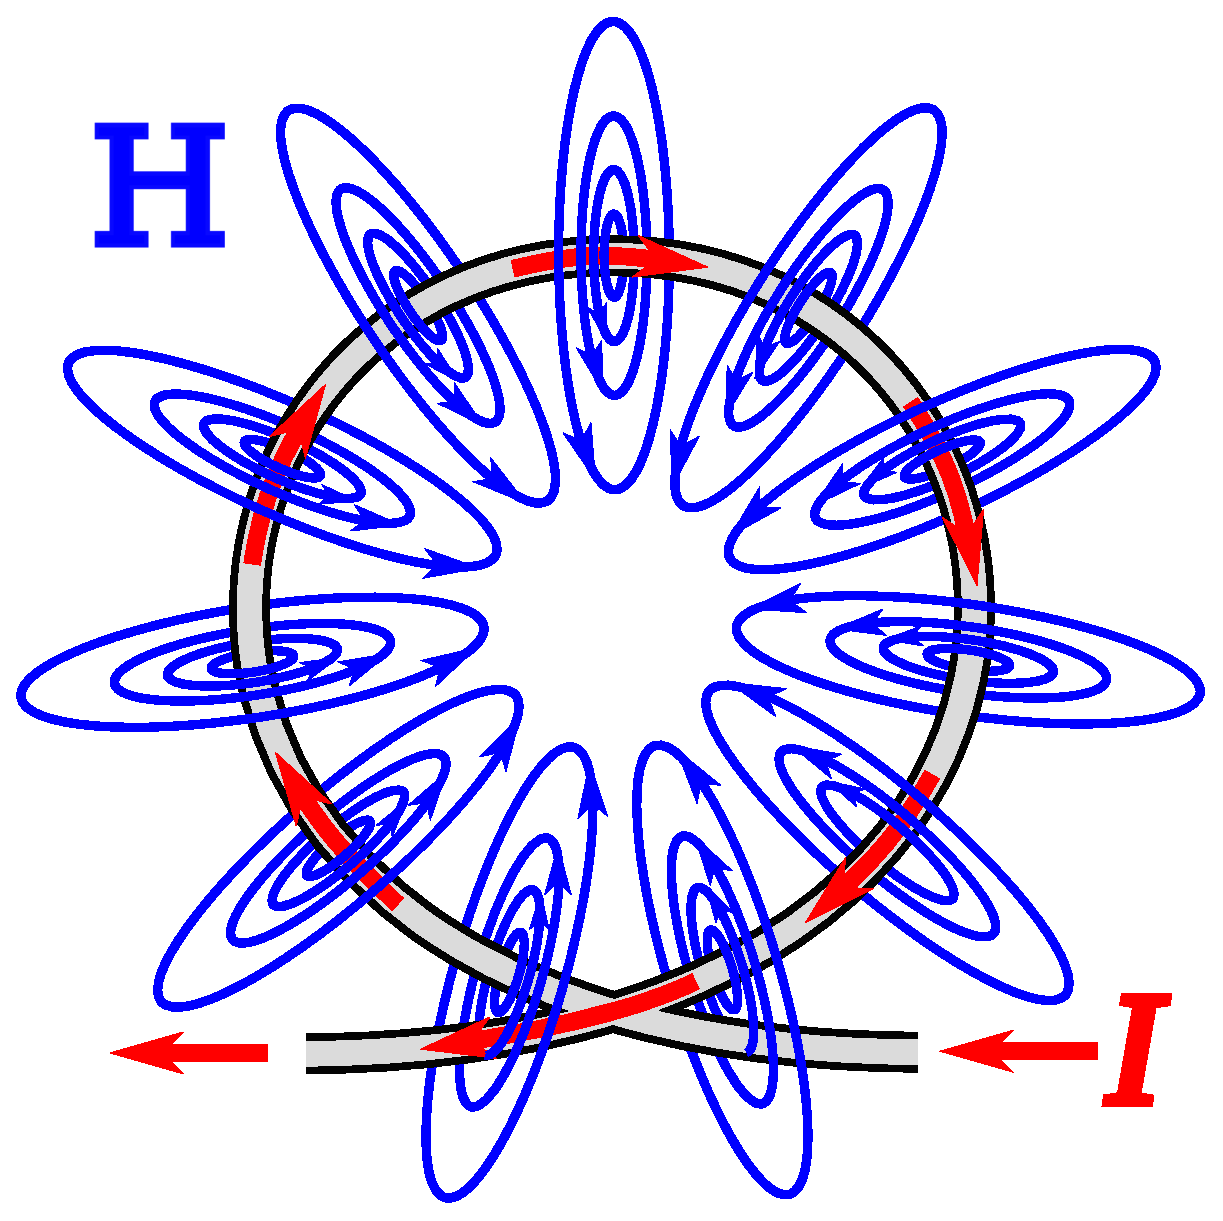
\includegraphics[width=2in]{modules/m0120_fOneTurn.eps}
% https://en.wikipedia.org/wiki/File:Magnetic_field_of_loop_3.svg
}}{A single loop of a coil. A dashed red line moves from the right entrance of the loop, around the loop, and out the left side exit, labeled I. Around the loop are 11 sets of blue concentric circles that represent magnetic fields, labeled H and spaced evenly. Each set has arrows on each concentric circle that point in toward the middle of the loop.}
\end{center} 
\centerline{\scriptsize 
\copyright~\hyperref[m0120_fOneTurn_Credit]{Chetvorno} 
\href{https://creativecommons.org/publicdomain/zero/1.0/deed.en}{CC0 1.0} (modified)
} 
\caption{
\label{m0120_fOneTurn}
Magnetic field due to a single loop.
}
\end{figure} 
 
Figure~\ref{m0120_fStraightCoilFieldLines}
also indicates that the magnetic field lines near the ends of the coil diverge from the axis of the coil.
This is understandable since magnetic field lines form closed loops.
The relatively complex structure of the magnetic fields near the ends of the coil (the ``fringing field'') 
\index{fringing (field)}
and outside of the coil make them relatively difficult to analyze.
Therefore, here we shall restrict our attention to the magnetic field deep inside the coil.
This restriction turns out to be of little consequence as long as $l\gg a$. 

Also, it is apparent from the radial symmetry of the coil that the magnitude of the magnetic field cannot depend on $\phi$.
Putting these findings together, we find that the most general form for the magnetic field intensity deep inside the coil is ${\bf H}\approx\hat{\bf z}H(\rho)$.  
That is, the direction of ${\bf H}$ is $\pm\hat{\bf z}$ and the magnitude of ${\bf H}$ depends, at most, on $\rho$.
In fact, we will soon find with the assistance of ACL that the magnitude of ${\bf H}$ doesn't depend on $\rho$ either.

Here's the relevant form of ACL:
%
\begin{equation}   
\oint_{\mathcal C}{ {\bf H} \cdot d{\bf l} } = I_{encl}  
\label{m0120_eACL}
\end{equation}
%
where $I_{encl}$ is the current enclosed by the closed path ${\mathcal C}$.
ACL works for {\it any} closed path that encloses the current of interest. 
Also, for simplicity, we prefer a path that lies on a constant-coordinate surface.
The selected path is shown in Figure~\ref{m0120_fPath}.
The benefits of this particular path will soon become apparent. 
However, note for now that this particular choice is consistent with the right-hand rule relating the direction of ${\mathcal C}$ to the direction of positive $I$.
That is, when $I$ is positive, the current in the turns of the coil pass through the surface bounded by ${\mathcal C}$ in the same direction as the fingers of the right hand when the thumb is aligned in the indicated direction of ${\mathcal C}$. 
%
\begin{figure}
\begin{center}
\pdftooltip{{  % note double braces
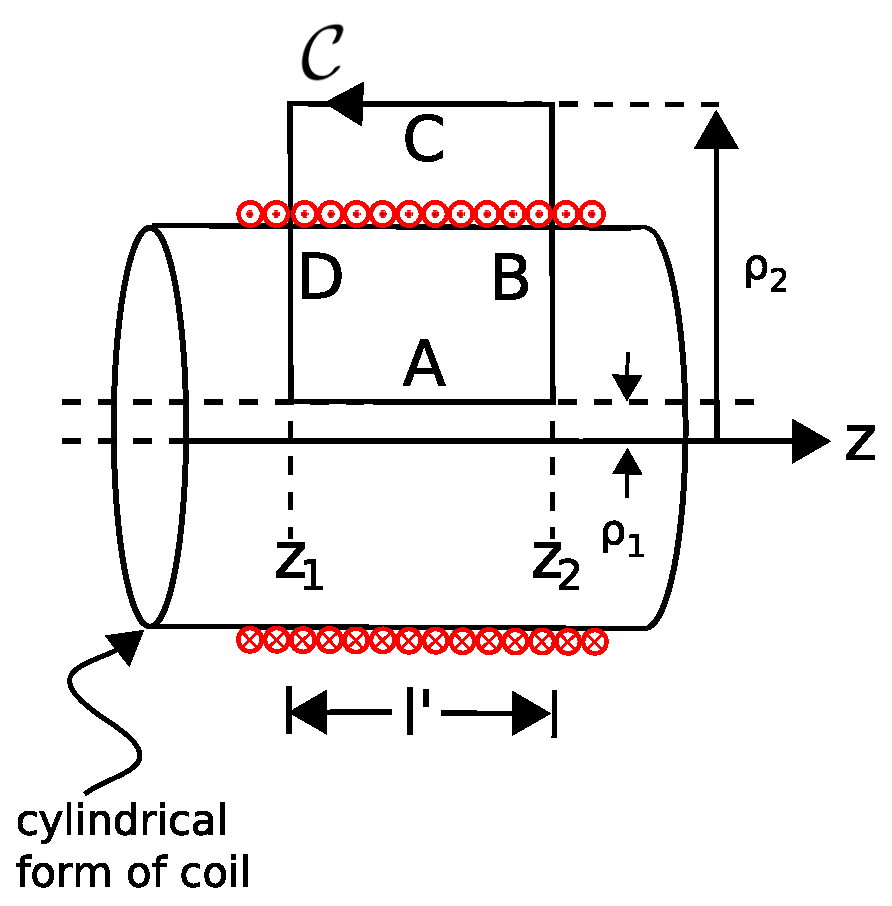
\includegraphics[width=2.5in]{modules/m0120_fPath.eps}
% https://commons.wikimedia.org/wiki/File:M0120_fPath.svg
}}{A cylindrical form of a coil, centered horizontally on the z-axis. On both sides of the cylinder are red circles; the top circles have dots in the middle, and the bottom circles have x’s. Laid over the top half of the cylinder is a square, with sides labeled A (bottom), B, C, and D in a counterclockwise direction creating a closed path, C, with counterclockwise direction. Corner DA is labeled Z sub 1. Corner AB is labeled z sub 2. Length of A is labeled l prime. Distance from z-axis to side C is rho sub 2. distance from z-axis to inner cylinder is rho 1. }
\end{center} 
\centerline{\scriptsize 
\copyright~\hyperref[m0120_fPath_Credit]{K.\ Kikkeri} 
\href{https://creativecommons.org/licenses/by-sa/4.0/}{CC BY~SA 4.0} 
} 
\caption{
\label{m0120_fPath}
Selected path of integration.
}
\end{figure}  

Let's define $N$ to be the number of windings in the coil.
Then, the winding density of the coil is $N/l$ (turns/m).
Let the path length in the $z$ direction be $l'$, as indicated in Figure~\ref{m0120_fPath}.
Then the enclosed current is
%
\begin{equation}
I_{encl}=\frac{N}{l}l'I
\end{equation}
%
That is, the number of turns per unit length times length gives number of turns, and
this quantity times the current through the wire is the total amount of current crossing the surface bounded by ${\mathcal C}$.
 
For the choice of ${\mathcal C}$ made above, and taking our approximation for the form of ${\bf H}$ as exact, Equation~\ref{m0120_eACL} becomes
%
\begin{equation}   
\oint_{\mathcal C}{ \left[\hat{\bf z}H(\rho)\right] \cdot d{\bf l} } = \frac{N}{l}l'I 
\label{m0120_eACL1}
\end{equation}
%
The integral consists of segments $A$, $B$, $C$, and $D$, as shown in Figure~\ref{m0120_fPath}.
Let us consider the result for each of these segments individually:
%
\begin{itemize}
\item The integral over segments $B$ and $D$ is zero because $d{\bf l}=\hat{\rho}d\rho$ for these segments, and so ${\bf H}\cdot d{\bf l}=0$ for these segments.
\item It is also possible to make the contribution from Segment~$C$ go to zero simply by letting $\rho_2\to\infty$.  
The argument is as follows. The magnitude of ${\bf H}$ outside the coil must decrease with distance from the coil, so for $\rho$ sufficiently large, ${\bf H}(\rho)$ becomes negligible.  If that's the case, then the integral over Segment~$C$ also becomes negligible.  
\end{itemize}
%
With $\rho_2\to\infty$, only Segment~$A$ contributes significantly to the integral over ${\mathcal C}$ and Equation~\ref{m0120_eACL1} becomes:
%
\begin{flalign}   
\frac{N}{l}l'I &= \int_{z_1}^{z_2}{ \left[\hat{\bf z}H(\rho_1)\right] \cdot \left(\hat{\bf z}dz\right) } \nonumber \\
               &= H(\rho_1) \int_{z_1}^{z_2}{ dz }                                                       \nonumber \\
               &= H(\rho_1) \left[ z_2-z_1 \right]                                                                    
\label{m0120_eACL2}
\end{flalign}
%
Note $z_2-z_1$ is simply $l'$. 
Also, we have found that the result is independent of $\rho_1$, as anticipated earlier. 
Summarizing:
%
\begin{equation}
\boxed{
{\bf H} \approx \hat{\bf z}\frac{NI}{l} ~~ \mbox{inside coil}
}
\label{m0120_eResult}
\end{equation}

Let's take a moment to consider the implications of this remarkably simple result.
%
\begin{itemize}
\item Note that it is dimensionally correct; that is, current divided by length gives units of A/m, which are the units of ${\bf H}$. 
\item We have found that the magnetic field is simply winding density ($N/l$) times current. To increase the magnetic field, you can either use more turns per unit length or increase the current.
\item We have found that the magnetic field is uniform inside the coil; that is, the magnetic field along the axis is equal to the magnetic field close to the cylinder wall formed by the coil.  However, this does not apply close to ends of the coil, since we have neglected the fringing field. 
\end{itemize}
%
These findings have useful applications in more complicated and practical problems, so it is worthwhile taking note of these now. Summarizing:
%
%ORB HIGHLIGHT
\begin{mdframed}[backgroundcolor=yellow!20,nobreak=true] 
The magnetic field deep inside an ideal straight coil (Equation~\ref{m0120_eResult}) is uniform and proportional to winding density and current.
\end{mdframed}

%------------------------------

{\bf Additional Reading:}
\begin{itemize}
\item ``\href{https://en.wikipedia.org/wiki/Electromagnetic_coil}{Electromagnetic Coil}'' on Wikipedia.
\item ``\href{https://en.wikipedia.org/wiki/Solenoid}{Solenoid}'' on Wikipedia.
\end{itemize}

\index{coil|)}



